\documentclass[11pt,a4paper]{report}
\usepackage[textwidth=37em,vmargin=30mm]{geometry}
\usepackage{calc,xunicode,amsmath,amssymb,paralist,enumitem,tabu,booktabs,datetime2,xeCJK,xeCJKfntef,listings}
\usepackage{tocloft,fancyhdr,tcolorbox,xcolor,graphicx,eso-pic,xltxtra,xelatexemoji}

\newcommand{\envyear}[0]{2025}
\newcommand{\envdatestr}[0]{2025-08-11}
\newcommand{\envfinaldir}[0]{webdb/2025/20250811/final}

\usepackage[hidelinks]{hyperref}
\hypersetup{
    colorlinks=false,
    pdfpagemode=FullScreen,
    pdftitle={Web Digest - \envdatestr}
}

\setlength{\cftbeforechapskip}{10pt}
\renewcommand{\cftchapfont}{\rmfamily\bfseries\large\raggedright}
\setlength{\cftbeforesecskip}{2pt}
\renewcommand{\cftsecfont}{\sffamily\small\raggedright}

\setdefaultleftmargin{2em}{2em}{1em}{1em}{1em}{1em}

\usepackage{xeCJK,xeCJKfntef}
\xeCJKsetup{PunctStyle=plain,RubberPunctSkip=false,CJKglue=\strut\hskip 0pt plus 0.1em minus 0.05em,CJKecglue=\strut\hskip 0.22em plus 0.2em}
\XeTeXlinebreaklocale "zh"
\XeTeXlinebreakskip = 0pt


\setmainfont{Brygada 1918}
\setromanfont{Brygada 1918}
\setsansfont{IBM Plex Sans}
\setmonofont{JetBrains Mono NL}
\setCJKmainfont{Noto Serif CJK SC}
\setCJKromanfont{Noto Serif CJK SC}
\setCJKsansfont{Noto Sans CJK SC}
\setCJKmonofont{Noto Sans CJK SC}

\setlength{\parindent}{0pt}
\setlength{\parskip}{8pt}
\linespread{1.15}

\lstset{
	basicstyle=\ttfamily\footnotesize,
	numbersep=5pt,
	backgroundcolor=\color{black!5},
	showspaces=false,
	showstringspaces=false,
	showtabs=false,
	tabsize=2,
	captionpos=b,
	breaklines=true,
	breakatwhitespace=true,
	breakautoindent=true,
	linewidth=\textwidth
}






\newcommand{\coverpic}[2]{
    % argv: itemurl, authorname
    Cover photo by #2~~(\href{#1}{#1})
}
\newcommand{\makeheader}[0]{
    \begin{titlepage}
        % \newgeometry{hmargin=15mm,tmargin=21mm,bmargin=12mm}
        \begin{center}
            
            \rmfamily\scshape
            \fontspec{BaskervilleF}
            \fontspec{Old Standard}
            \fontsize{59pt}{70pt}\selectfont
            WEB\hfill DIGEST
            
            \vfill
            % \vskip 30pt
            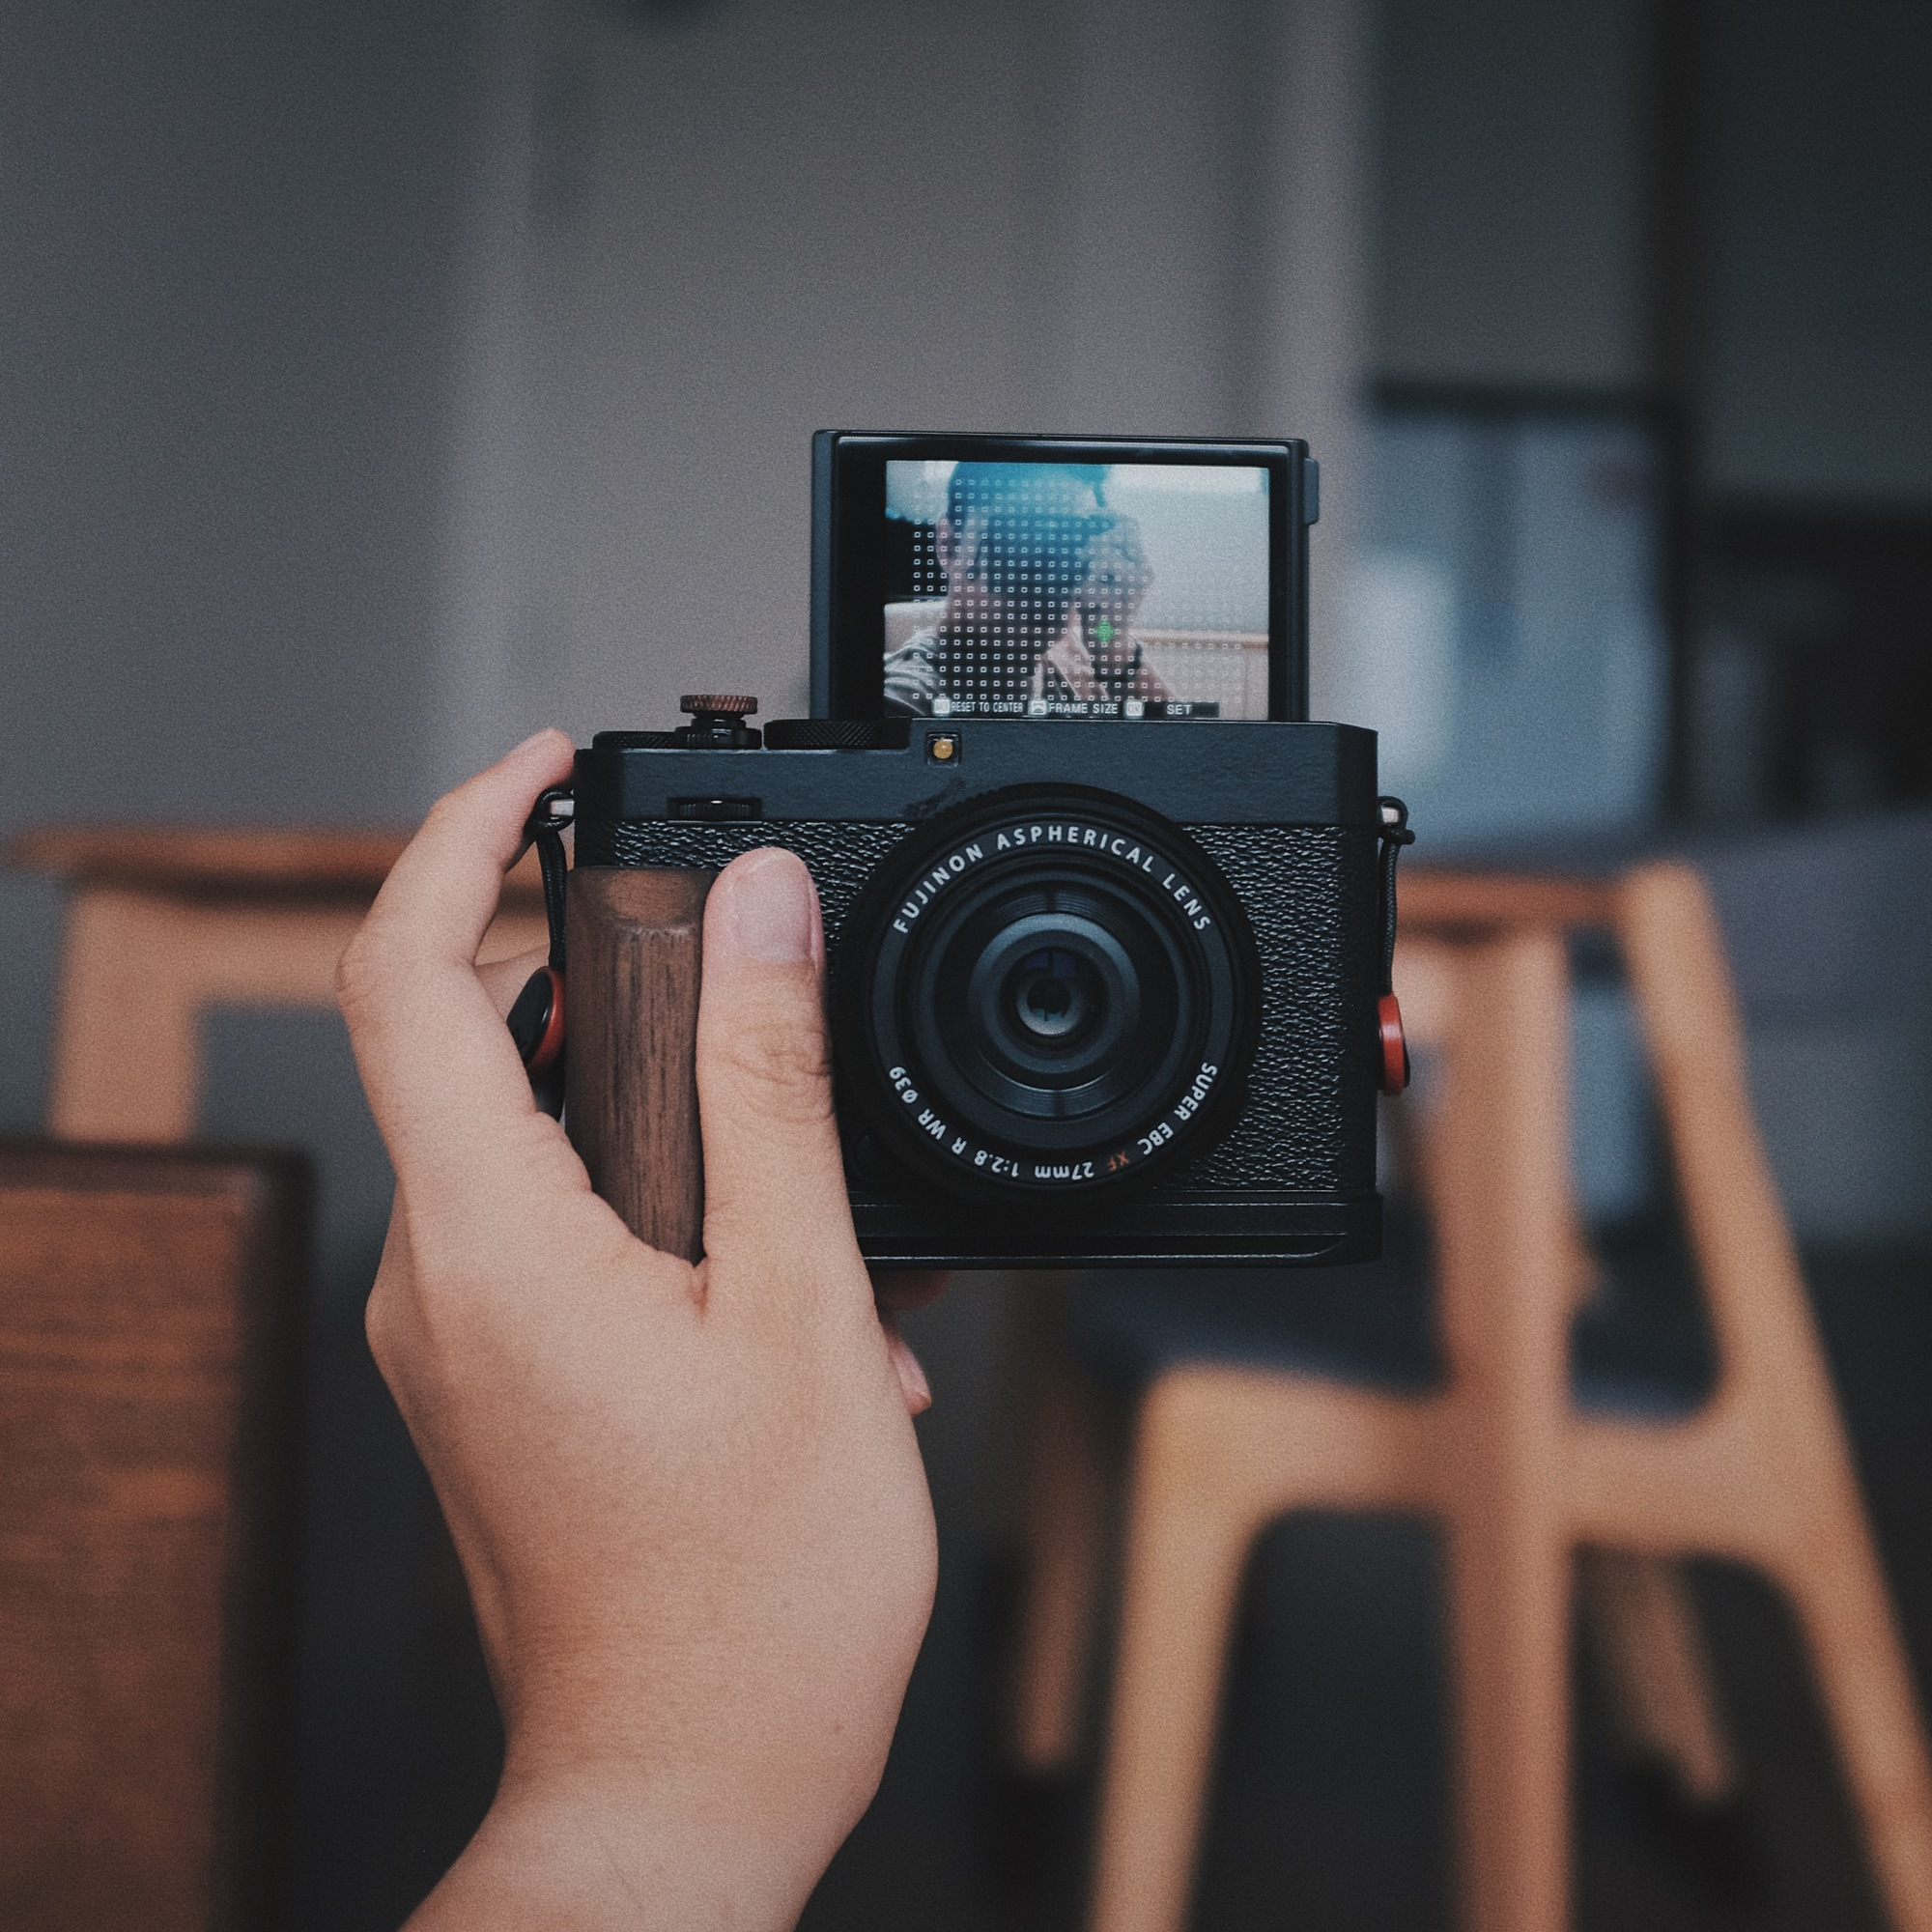
\includegraphics[width=\linewidth]{\envfinaldir/coverpic-prod.jpg}\par
            % \vskip 30pt
            \vfill

            \normalsize\rmfamily\scshape
            \copyright{} The Web Digest Project \hfill\large \envdatestr
        \end{center}
    \end{titlepage}
    % \restoregeometry
}
\newcommand{\simplehref}[1]{%
    \textcolor{blue!80!green}{\href{#1}{#1}}%
}
\renewcommand{\contentsname}{\center\Huge\sffamily\bfseries Contents\par\vskip 20pt}
\newcounter{ipartcounter}
\setcounter{ipartcounter}{0}
\newcommand{\ipart}[1]{
    % \vskip 20pt
    \clearpage
    \stepcounter{ipartcounter}
    \phantomsection
    \addcontentsline{toc}{chapter}{#1}
    % \begin{center}
    %     \Huge
    %     \sffamily\bfseries
    %     #1
    % \end{center}
    % \vskip 20pt plus 7pt
}
\newcounter{ichaptercounter}
\setcounter{ichaptercounter}{0}
\newcommand{\ichapter}[1]{
    % \vskip 20pt
    \clearpage
    \stepcounter{ichaptercounter}
    \phantomsection
    \addcontentsline{toc}{section}{\numberline{\arabic{ichaptercounter}}#1}
    \begin{center}
        \Huge
        \sffamily\bfseries
        #1
    \end{center}
    \vskip 20pt plus 7pt
}
\newcommand{\entrytitlefont}[1]{\subsection*{\raggedright\Large\sffamily\bfseries#1}}
\newcommand{\entryitemGeneric}[2]{
    % argv: title, url
    \parbox{\linewidth}{
        \entrytitlefont{#1}\par\vskip 5pt
        \footnotesize\ttfamily\mdseries
        \simplehref{#2}
    }\vskip 11pt plus 11pt minus 1pt
}
\newcommand{\entryitemGithub}[3]{
    % argv: title, url, desc
    \parbox{\linewidth}{
        \entrytitlefont{#1}\par\vskip 5pt
        \footnotesize\ttfamily\mdseries
        \simplehref{#2}\par\vskip 5pt
        \small\rmfamily\mdseries#3
    }\vskip 11pt plus 11pt minus 1pt
}
\newcommand{\entryitemAp}[3]{
    % argv: title, url, desc
    \parbox{\linewidth}{
        \entrytitlefont{#1}\par\vskip 5pt
        \footnotesize\ttfamily\mdseries
        \simplehref{#2}\par\vskip 5pt
        \small\rmfamily\mdseries#3
    }\vskip 11pt plus 11pt minus 1pt
}
\newcommand{\entryitemHackernews}[3]{
    % argv: title, hnurl, rawurl
    % \parbox{\linewidth}{
    %     \entrytitlefont{#1}\par\vskip 5pt
    %     \footnotesize\ttfamily\mdseries
    %     \simplehref{#3}\par
    %     \textcolor{black!50}{\href{#2}{#2}}
    % }\vskip 11pt plus 11pt minus 1pt
    \begin{minipage}{\linewidth}
            \entrytitlefont{#1}\par\vskip 5pt
            \footnotesize\ttfamily\mdseries
            \simplehref{#3}\par
            \textcolor{black!50}{\href{#2}{#2}}
    \end{minipage}\par\vskip 11pt plus 11pt minus 1pt
}







\begin{document}

\makeheader

\tableofcontents\clearpage




\ipart{Developers}
\ichapter{Hacker News}
\entryitemTwoLinks{1910: The year the modern world lost its mind}{https://news.ycombinator.com/item?id=44858154}{https://www.derekthompson.org/p/1910-the-year-the-modern-world-lost}

\entryitemTwoLinks{Show HN: Bolt – A super-fast, statically-typed scripting language written in C}{https://news.ycombinator.com/item?id=44856935}{https://github.com/Beariish/bolt}

\entryitemTwoLinks{Fight Chat Control}{https://news.ycombinator.com/item?id=44856426}{https://fightchatcontrol.eu/}

\entryitemTwoLinks{Diffusion language models are super data learners}{https://news.ycombinator.com/item?id=44856101}{https://jinjieni.notion.site/Diffusion-Language-Models-are-Super-Data-Learners-239d8f03a866800ab196e49928c019ac}

\entryitemTwoLinks{AOL closes its dial up internet service}{https://news.ycombinator.com/item?id=44856090}{https://www.ispreview.co.uk/index.php/2025/08/after-34-years-aol-finally-closes-its-dial-up-internet-service.html}

\entryitemTwoLinks{Zig's Lovely Syntax}{https://news.ycombinator.com/item?id=44855881}{https://matklad.github.io/2025/08/09/zigs-lovely-syntax.html}

\entryitemTwoLinks{GPT-OSS vs. Qwen3 and a detailed look how things evolved since GPT-2}{https://news.ycombinator.com/item?id=44855690}{https://magazine.sebastianraschka.com/p/from-gpt-2-to-gpt-oss-analyzing-the}

\entryitemTwoLinks{Show HN: Engineering.fyi – Search across tech engineering blogs in one place}{https://news.ycombinator.com/item?id=44855157}{https://engineering.fyi/}

\entryitemTwoLinks{Try and}{https://news.ycombinator.com/item?id=44855079}{https://ygdp.yale.edu/phenomena/try-and}

\entryitemTwoLinks{MCP: An (Accidentally) Universal Plugin System}{https://news.ycombinator.com/item?id=44854860}{https://worksonmymachine.ai/p/mcp-an-accidentally-universal-plugin}

\entryitemTwoLinks{Booting 5000 Erlangs on Ampere One 192-core}{https://news.ycombinator.com/item?id=44854525}{https://underjord.io/booting-5000-erlangs-on-ampere-one.html}

\entryitemTwoLinks{Open Lovable}{https://news.ycombinator.com/item?id=44854120}{https://github.com/mendableai/open-lovable}

\entryitemTwoLinks{Writing simple tab-completions for Bash and Zsh}{https://news.ycombinator.com/item?id=44854035}{https://mill-build.org/blog/14-bash-zsh-completion.html}

\entryitemTwoLinks{Abogen – Generate audiobooks from EPUBs, PDFs and text}{https://news.ycombinator.com/item?id=44853064}{https://github.com/denizsafak/abogen}

\entryitemTwoLinks{Melonking Website}{https://news.ycombinator.com/item?id=44852582}{https://melonking.net/}

\entryitemTwoLinks{Happy BuyNothing Day}{https://news.ycombinator.com/item?id=44851590}{https://justbuynothing.com/}

\entryitemTwoLinks{GPT-5: Overdue, overhyped and underwhelming. And that's not the worst of it}{https://news.ycombinator.com/item?id=44851557}{https://garymarcus.substack.com/p/gpt-5-overdue-overhyped-and-underwhelming}

\entryitemTwoLinks{GPTs and Feeling Left Behind}{https://news.ycombinator.com/item?id=44851214}{https://whynothugo.nl/journal/2025/08/06/gpts-and-feeling-left-behind/}

\entryitemTwoLinks{How I code with AI on a budget/free}{https://news.ycombinator.com/item?id=44850913}{https://wuu73.org/blog/aiguide1.html}

\entryitemTwoLinks{Abusing Entra OAuth for fun and access to internal Microsoft applications}{https://news.ycombinator.com/item?id=44850681}{https://research.eye.security/consent-and-compromise/}\ichapter{Phoronix}
\entryitemGeneric{\hskip 0pt{}Linux 6.17-rc1 Released With Many New Features But No Bcachefs Changes}{https://www.phoronix.com/news/Linux-6.17-rc1}

\entryitemGeneric{\hskip 0pt{}Debian 14 Eyes LoongArch CPU Support}{https://www.phoronix.com/news/Debian-14-Loong64-LoongArch}

\entryitemGeneric{\hskip 0pt{}GNOME Shell 49 Beta Finally Brings Media Controls To The Lock Screen}{https://www.phoronix.com/news/GNOME-Shell-Meda-Lock-Screen}

\entryitemGeneric{\hskip 0pt{}Turbostat Now Displays CPU L3 Cache Topology Information}{https://www.phoronix.com/news/Linux-6.17-Turbostat}

\entryitemGeneric{\hskip 0pt{}Btrfs Has Saved Meta "Billions Of Dollars" In Infrastructure Costs}{https://www.phoronix.com/news/Btrfs-Saves-Meta-Billions}

\entryitemGeneric{\hskip 0pt{}Debian 13.0 "Trixie" Now Available - Powered By Linux 6.12 LTS}{https://www.phoronix.com/news/Debian-13.0-Released}

\entryitemGeneric{\hskip 0pt{}Linux 6.17 EFI Stub Will Try To Maintain a Cleaner Boot Experience}{https://www.phoronix.com/news/Linux-6.17-EFI-Stub-Clean-Boot}

\entryitemGeneric{\hskip 0pt{}Vulkan 1.4.325 Released With Untyped Pointers Extension}{https://www.phoronix.com/news/Vulkan-1.4.325-Released}

\entryitemGeneric{\hskip 0pt{}Linus Torvalds Rejects RISC-V Changes For Linux 6.17: "Garbage"}{https://www.phoronix.com/news/Linux-6.17-RISC-V-Rejected}


\ipart{Developers~~~~(zh-Hans)}
\ichapter{Solidot}
\entryitemGeneric{\hskip 0pt{}Debian 13 trixie 释出}{https://www.solidot.org/story?sid=82003}

\entryitemGeneric{\hskip 0pt{}AI 淘汰初级编程开发者}{https://www.solidot.org/story?sid=82002}

\entryitemGeneric{\hskip 0pt{}签署捐赠誓言的 256 名亿万富翁只有 9 人信守诺言 }{https://www.solidot.org/story?sid=82001}

\entryitemGeneric{\hskip 0pt{}科学家研发能针对多种病毒的通用疫苗}{https://www.solidot.org/story?sid=82000}

\entryitemGeneric{\hskip 0pt{}Google 发现了一种新骗局,随后自己成为了该骗局的受害者}{https://www.solidot.org/story?sid=81999}

\entryitemGeneric{\hskip 0pt{}一颗大质量白矮星被发现是由双星合并而成}{https://www.solidot.org/story?sid=81998}

\entryitemGeneric{\hskip 0pt{}中国工程师解决磁悬浮列车的隧道微压波噪音}{https://www.solidot.org/story?sid=81997}

\entryitemGeneric{\hskip 0pt{}中国主要太阳能公司去年裁员近三分之一}{https://www.solidot.org/story?sid=81994}

\entryitemGeneric{\hskip 0pt{}Windows 10 的 30 美元扩展安全更新支持单一账号 10 台设备}{https://www.solidot.org/story?sid=81993}

\entryitemGeneric{\hskip 0pt{}Linux 桌面市场份额达到 6\%}{https://www.solidot.org/story?sid=81992}

\entryitemGeneric{\hskip 0pt{}OpenAI 发布 GPT-5}{https://www.solidot.org/story?sid=81991}

\entryitemGeneric{\hskip 0pt{}科学家重新创造宇宙第一种分子}{https://www.solidot.org/story?sid=81990}\ichapter{V2EX}
\entryitemGeneric{\hskip 0pt{}[macOS] 有没有人发现 macOS 26 的 ChatGPT 状态栏图标消失了}{https://www.v2ex.com/t/1151430}

\entryitemGeneric{\hskip 0pt{}[问与答] 觉得 claude code 很差劲是政治不正确吗?}{https://www.v2ex.com/t/1151429}

\entryitemGeneric{\hskip 0pt{}[问与答] tailscale 配置子网互访,参考 Site-to-site networking 的问题咨询}{https://www.v2ex.com/t/1151428}

\entryitemGeneric{\hskip 0pt{}[问与答] Apple 的密码应用现在如何?能不能取代 1Password?}{https://www.v2ex.com/t/1151427}

\entryitemGeneric{\hskip 0pt{}[推广] 又送 u 了,搞活动了}{https://www.v2ex.com/t/1151426}

\entryitemGeneric{\hskip 0pt{}[问与答] 要处理不是本人行驶证的车扣分,可以在 app 操作还是要去交警处理}{https://www.v2ex.com/t/1151425}

\entryitemGeneric{\hskip 0pt{}[V2EX] 忽略 solana 节点后,世界清净了……}{https://www.v2ex.com/t/1151424}

\entryitemGeneric{\hskip 0pt{}[VXNA] 申请收录个人博客 https://ysx.cosine.ren/}{https://www.v2ex.com/t/1151423}

\entryitemGeneric{\hskip 0pt{}[ WATCH] 想入手一款 iwatch,请各位推荐几款,最好能阐明优劣势,感谢}{https://www.v2ex.com/t/1151422}

\entryitemGeneric{\hskip 0pt{}[问与答] 磷酸铁锂的电芯 diy 电瓶车电池可以么?}{https://www.v2ex.com/t/1151421}

\entryitemGeneric{\hskip 0pt{}[酷工作] [社招] [北京] 多邻国 Duolingo 招聘 Senior Platform Engineer - Infrastructure Platform}{https://www.v2ex.com/t/1151419}

\entryitemGeneric{\hskip 0pt{}[程序员] 搜了下华为 100w 充电器 结果有点震惊}{https://www.v2ex.com/t/1151418}

\entryitemGeneric{\hskip 0pt{}[宽带症候群] 经过查询宽带测试的国标标准得出以下结论}{https://www.v2ex.com/t/1151417}

\entryitemGeneric{\hskip 0pt{}[程序员] Qwen MT 翻译尽然有这么严格的敏感信息审查}{https://www.v2ex.com/t/1151416}

\entryitemGeneric{\hskip 0pt{}[信息安全] 把 Clash RCE 武器化的典型案例}{https://www.v2ex.com/t/1151415}

\entryitemGeneric{\hskip 0pt{}[Solana] \$V2EX が LBank に上場決定!}{https://www.v2ex.com/t/1151414}

\entryitemGeneric{\hskip 0pt{}[酷工作] 招聘: PM+前端工程师 Rust 开发工程师-Rust 交易系统方向 UI/UX 设计师 中台交易监控的开发架构 或者经理 或者资深开发 谷歌 SEO 优化师 全球人力资源与组织运营负责人(支持去中心化组织转型)}{https://www.v2ex.com/t/1151411}

\entryitemGeneric{\hskip 0pt{}[分享创造] 不想再手动复制,我做了一个 pdf 批量导入飞书的工具,格式图片都还原那种}{https://www.v2ex.com/t/1151410}

\entryitemGeneric{\hskip 0pt{}[问与答] 小米平板 5pro 碎屏了, 自己换靠谱不?}{https://www.v2ex.com/t/1151409}

\entryitemGeneric{\hskip 0pt{}[程序员] 雷霆是跑路了吗? 节点都挂了}{https://www.v2ex.com/t/1151408}

\entryitemGeneric{\hskip 0pt{}[旅行] 东京独自旅行游记}{https://www.v2ex.com/t/1151406}

\entryitemGeneric{\hskip 0pt{}[OpenAI] 感觉 GPT-5 智障了}{https://www.v2ex.com/t/1151405}

\entryitemGeneric{\hskip 0pt{}[问与答] 各位大神,有没有什么办法能解决将手机 iPhone 或 android 或者是 win 电脑同时投屏到多台电视上,都在同一局域网下,有线太麻烦,有没有好办法?}{https://www.v2ex.com/t/1151404}

\entryitemGeneric{\hskip 0pt{}[OpenAI] 我感觉 GPT-5 并没有想象中的那么强}{https://www.v2ex.com/t/1151403}

\entryitemGeneric{\hskip 0pt{}[程序员] AI 主导项目需求开发最佳实践[咨询]}{https://www.v2ex.com/t/1151402}

\entryitemGeneric{\hskip 0pt{}[Steam] 关于 Steam Deck 原生系统使用代理工具 V2RayN}{https://www.v2ex.com/t/1151401}

\entryitemGeneric{\hskip 0pt{}[VPS] 避雷 LisaHost 丽萨主机|第一次知道还有 [共享带宽] 这种卖法}{https://www.v2ex.com/t/1151400}

\entryitemGeneric{\hskip 0pt{}[电影] 2025 年暑假档的电影基本都看了}{https://www.v2ex.com/t/1151399}

\entryitemGeneric{\hskip 0pt{}[宽带症候群] 光猫更换猫棒能避免运营商控制吗}{https://www.v2ex.com/t/1151398}

\entryitemGeneric{\hskip 0pt{}[程序员] 像写代码一样设计你的 Prompt,实现 Prompt As Code。}{https://www.v2ex.com/t/1151396}

\entryitemGeneric{\hskip 0pt{}[问与答] 想讲一讲自己这么多年的创伤,大家觉得是矫情吗?}{https://www.v2ex.com/t/1151394}

\entryitemGeneric{\hskip 0pt{}[分享创造] 个人开源项目:小红书 MCP,完成小红书自动化运营}{https://www.v2ex.com/t/1151393}

\entryitemGeneric{\hskip 0pt{}[程序员] 外包领导决策失误,导致整个部门被清场一大半,其中就有我。}{https://www.v2ex.com/t/1151390}

\entryitemGeneric{\hskip 0pt{}[问与答] 请网络大佬帮忙解答下}{https://www.v2ex.com/t/1151389}

\entryitemGeneric{\hskip 0pt{}[程序员] grpc gateway 存在的意义是什么}{https://www.v2ex.com/t/1151388}

\entryitemGeneric{\hskip 0pt{}[推广] 两天时间搭建了自用推特视频下载服务分享}{https://www.v2ex.com/t/1151387}

\entryitemGeneric{\hskip 0pt{}[Solana] 如果想做一个和\$v2ex 联动的 web app,应该如何入手?}{https://www.v2ex.com/t/1151386}

\entryitemGeneric{\hskip 0pt{}[Linux] 提醒拿 vanilla Debian 做路由器的, Trixie 下的 miniupnpd 可能有问题}{https://www.v2ex.com/t/1151385}

\entryitemGeneric{\hskip 0pt{}[微信] 微信怎么回事?一直在改我的通知显示内容设置}{https://www.v2ex.com/t/1151383}

\entryitemGeneric{\hskip 0pt{}[Solana] 使用 okx web3 查看\$v2ex 信息}{https://www.v2ex.com/t/1151382}

\entryitemGeneric{\hskip 0pt{}[VPS] xray fallback 问题,有偿 100 块,速来。}{https://www.v2ex.com/t/1151381}

\entryitemGeneric{\hskip 0pt{}[生活] 准备添置一台 27 寸 4k 显示器,有什么推荐吗}{https://www.v2ex.com/t/1151377}

\entryitemGeneric{\hskip 0pt{}[Linux] 服务器已经升级到 Debian 13 了}{https://www.v2ex.com/t/1151375}

\entryitemGeneric{\hskip 0pt{}[分享创造] 用 AI 写的开源高性能远程桌面软件}{https://www.v2ex.com/t/1151374}

\entryitemGeneric{\hskip 0pt{}[OpenAI] GPT5 怎么那么喜欢画图?}{https://www.v2ex.com/t/1151373}

\entryitemGeneric{\hskip 0pt{}[以太坊] 以太坊十周年纪念 NFT 地板价 5.01U}{https://www.v2ex.com/t/1151372}

\entryitemGeneric{\hskip 0pt{}[求职] 双非本科,工作三年,迷茫了。现在面临一个选择,是考编制,还是要钱。}{https://www.v2ex.com/t/1151369}

\entryitemGeneric{\hskip 0pt{}[分享创造] 告别静态 neofetch,用 neonfetch 点亮终端}{https://www.v2ex.com/t/1151368}

\entryitemGeneric{\hskip 0pt{}[Solana] \$V2EX 转 SOL 短网址}{https://www.v2ex.com/t/1151367}

\entryitemGeneric{\hskip 0pt{}[分享创造] [小程序] 做了一个帮我决定周末去哪的小程序}{https://www.v2ex.com/t/1151365}


\ipart{Generic News}







\clearpage
\leavevmode\vfill
\footnotesize

Copyright \copyright{} 2023-2025 Neruthes and other contributors.

This document is published with CC BY-NC-ND 4.0 license.

The entries listed in this newsletter may be copyrighted by their respective creators.

This newsletter is generated by the Web Digest project.

The newsletters are also delivered via Telegram channel \CJKunderline{\href{https://t.me/webdigestchannel}{https://t.me/webdigestchannel}}.\\
RSS feed is available at \CJKunderline{\href{https://webdigest.pages.dev/rss.xml}{https://webdigest.pages.dev/rss.xml}}.

This newsletter is available in PDF at
\CJKunderline{\href{https://webdigest.pages.dev/}{https://webdigest.pages.dev/}}.

The source code being used to generate this newsletter is available at\\
\CJKunderline{\href{https://github.com/neruthes/webdigest}{https://github.com/neruthes/webdigest}}.

This newsletter is also available in
\CJKunderline{\href{http://webdigest.pages.dev/readhtml/\envyear/WebDigest-20250811.html}{HTML}} and
\CJKunderline{\href{https://github.com/neruthes/webdigest/blob/master/markdown/\envyear/WebDigest-20250811.md}{Markdown}}.


\coverpic{}{}


\end{document}
